\begin{frame}{Nearest Neighbour}
\begin{columns}
		\begin{column}{0.6\textwidth}
	\begin{itemize}
		\item Nearest Neighbour wurde so implementiert, dass das Programm die Lösungen für alle Startpunkte miteinander vergleicht und die beste auswählt.
        \item Grundsätzliche Vorgangsweise:
    \end{itemize}
    \begin{enumerate}
     	\item Startknoten zufällig wählen
        \item Knoten mit geringster Entfernung zu aktuellem Knoten wird in Tour aufgenommen.
        \item Wiederhole Schritt 2 bis nur noch die Verbindung zum Startknoten übrig bleibt.
        \item Verbinde den zuletzt hinzugefügten Knoten mit dem Startknoten.
	\end{enumerate}
    	\end{column}
        \begin{column}{0.4\textwidth}
        \begin{figure} 
        	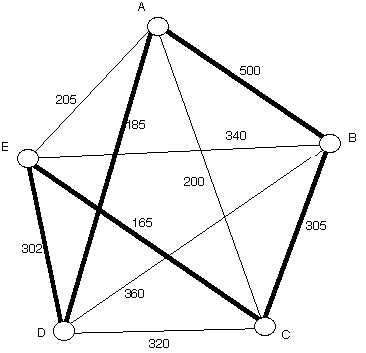
\includegraphics[scale=0.30]{NN.png}
            starting in node A
        \end{figure}
  	  \end{column}
  \end{columns}
\end{frame}

\begin{frame}{Nearest/Cheapest Insertion}
\begin{columns}
	  \begin{column}{0.45\textwidth}
	\begin{itemize}
		\item Vorgehen bei beiden Heuristiken gleich.
      	\item Unterschied liegt alleine im Insertionkriterium.
	\begin{enumerate}
       	\item Starte mit 2 Knoten.
        \item Einfügen des nächsten Knoten nach Auswahlkriterium:
        	\begin{itemize}
            	\item Nearest $\Rightarrow$ Knoten mit kürzester Entfernung
            	\item Cheapest $\Rightarrow$ Knoten mit geringsten Einfügekosten
            \end{itemize}
        \item Wiederhole Schritt 2 bis alle Knoten Teil der Tour sind.
        \end{enumerate}
	\end{itemize}
	  \end{column}
      \begin{column}{0.55\textwidth}
        \begin{figure} 
        	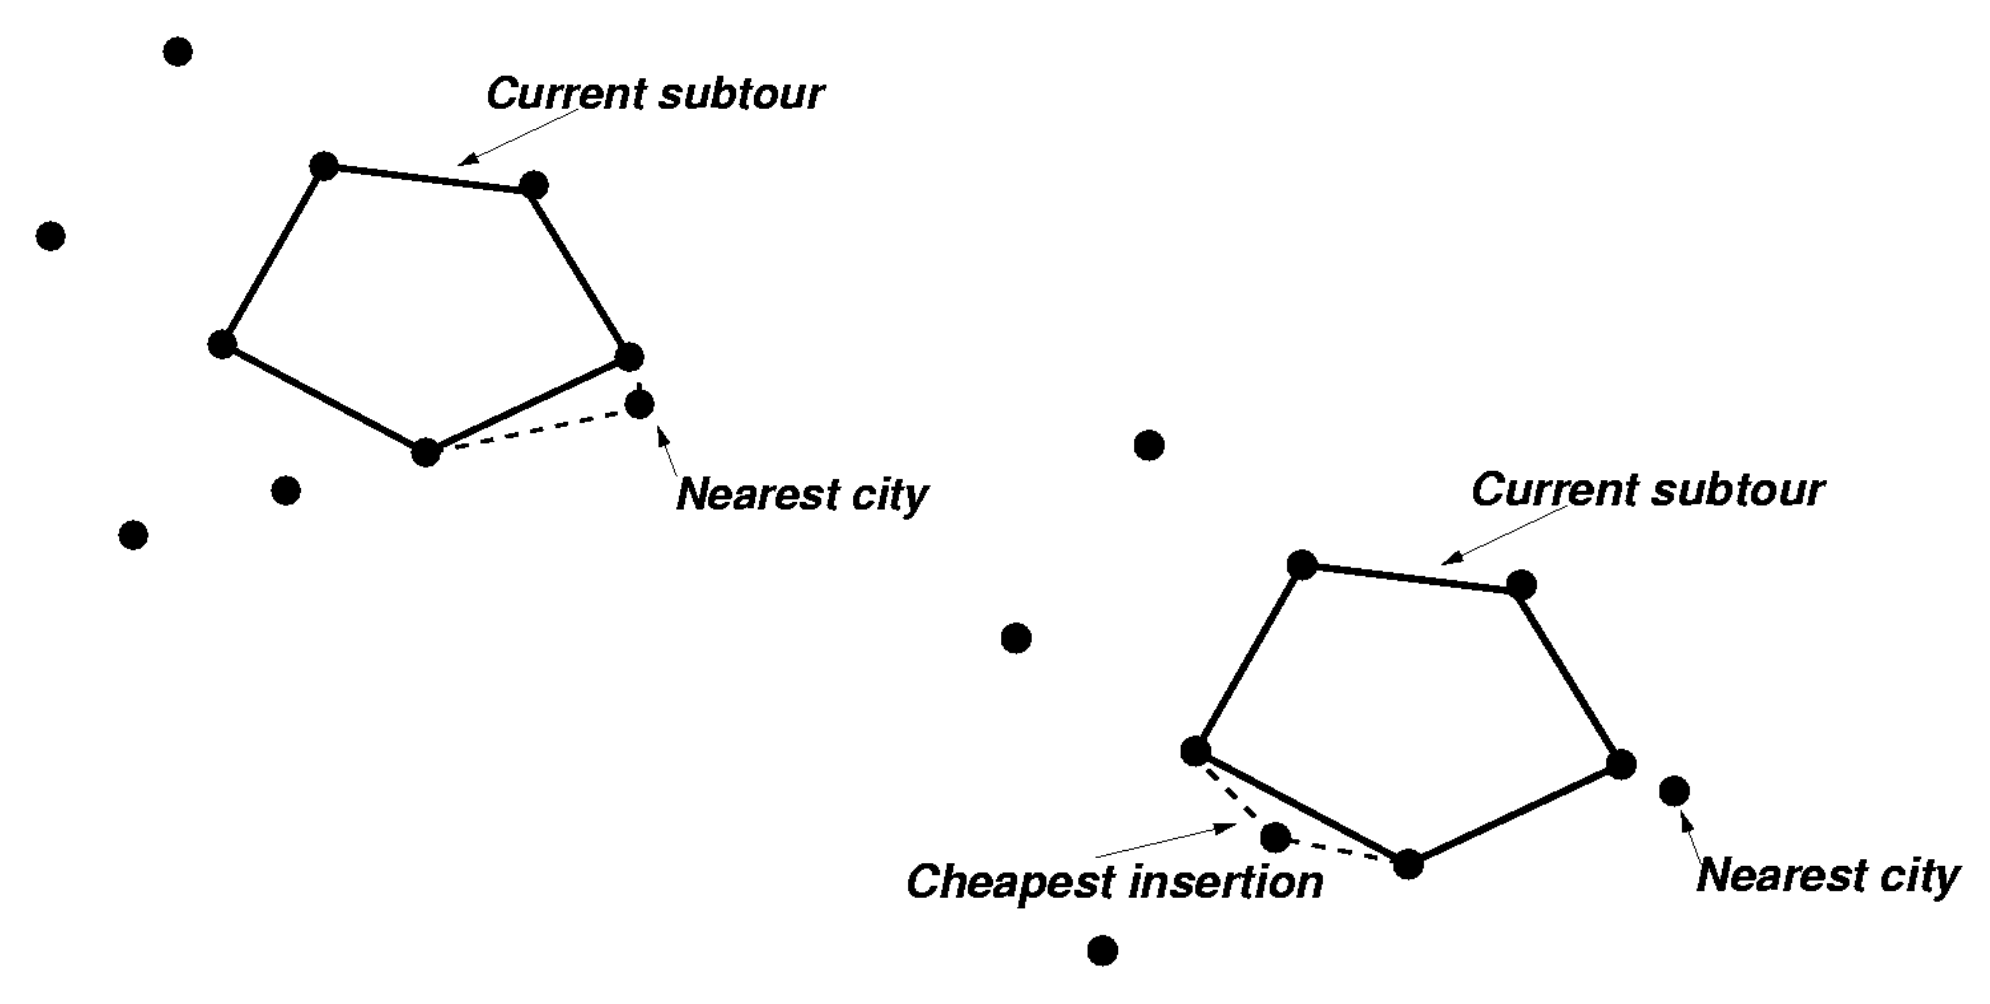
\includegraphics[scale=0.20]{NICI.png}
        \end{figure}
  	  \end{column}
  \end{columns}
\end{frame}